%============================================================
% 	Theme		::	`tutorial' Beamer Theme
%					-- BASED on Szeged (Till Tantau)
%					----------------------------------------
%	Color		::	Self-Contained
%					-- mainly `whale' Beamer Color Theme
%					-- with Rich Black, Beach Pink & Teal
%					----------------------------------------
%	Font		::	Fira Sans Beamer Font Theme
%					-- Mozilla's Fira Sans Typeface
%					-- FROM Metropolis (Matthias Vogelgesang)
%					-- use XeLaTeX for better visual effects
%					----------------------------------------
%	Author		::	Xu, Minjie (Jeff)
%	Created		::	2016-02-10
%	Updated		::	March 28, 2016 at 02:51AM (CST)
%	Version		::	1.0.1
%	Contact		::	GitHub.com/jeffmxu
%					-----------------------------------------
% 	License		::	LPPL 1.3c or later
%					GNU GPLv4 or later
%					CC-BY-SA 4.0 or later
% 	Notice		::	Copyright 2016 XU Minjie (Jeff)
%					This `tutorial' beamer theme presentation may be distributed and/or modified under the LaTeX Project Public License (version 1.3 or later) and/or under the GNU General Public License (version 3.0 or later).
%					This `tutorial' beamer theme presentation is also required to be licensed under the Creative Commons Attribution-ShareAlike 4.0 International License (or any later version).
%					-----------------------------------------
%	Description	::	This presentation is a demonstration of `tutorial' beamer theme, which is INFLUENCED by Metropolis from Matthias Vogelgesang (GitHub.com/matze) and BASED on Szeged with `whale' color theme of Till Tantau.
%============================================================



%============================================================
%	THEME, OPTIONS & PACKAGES
%------------------------------------------------------------
%\ProcessOptionsToClass{dvipsnames, svgnames, xl1names, table}{beamer}
\documentclass{beamer}%[dvipsnames, svgnames, xl1names, table]
\usetheme[light, minimal]{tutorial}%[light, minimal]
%\setbeamercolor{structure}{fg=Maroon}% keep background WHITE
%------------------------------------------------------------
% uncover everything in a step-wise fashion
%\beamerdefaultoverlayspecification{<+->}
%------------------------------------------------------------
\usepackage[scale=1.618]{ccicons}
\usepackage{listings, subcaption}
\lstset{language=[LaTeX]TeX,basicstyle=\ttfamily}
\captionsetup[sub]{font+=scriptsize,labelformat=simple,labelsep=quad}
%------------------------------------------------------------
\newcommand{\theme}{\texttt{tutorial}}
%============================================================



%============================================================
%	PRESENTATION INFORMATION
%------------------------------------------------------------
\title[Title]{\theme}% v0.3.5
\subtitle[Subtitle]{A light Beamer theme for academics}
\author[Author]{Jeff M Xu}
\institute[Institute]{\href{https://github.com/jeffmxu}{\texttt{github.com/jeffmxu}}}
%------------------------------------------------------------
\hypersetup{%
	pdfkeywords	= {beamer, demo, theme, tutorial},
	pdfcreator	= {MiKTeX-XeTeX 2.9.5840 (64-bit)},% Windows OS
}
%============================================================



%============================================================
%	TITLE PAGE & OUTLINE
%------------------------------------------------------------
\begin{document}
\begin{frame}
	\maketitle% recommend to be framed only for DEFAULT style
\end{frame}
%------------------------------------------------------------
\begin{frame}{Outline}
	\tableofcontents%[pausesections]?
\end{frame}
%============================================================



%============================================================
%	INTRODUCTION
%------------------------------------------------------------
\section{Introduction}
%------------------------------------------------------------
%\subsection{\theme\ and Options}
%------------------------------------------------------------
\begin{frame}{\theme}
\begin{itemize}
\item A light modern Beamer theme with\ldots
	\begin{itemize}
	\item flat style based on Szeged
	\item energetic text colors
	\item \texttt{light} or \texttt{minimal} visual noise
	\end{itemize}
\item Adjusted for academics with\ldots
	\begin{itemize}
	\item traditional \textcolor{BlendedBlue}{blended blue} $\times$ white \texttt{whale} color theme
	\item maximized frame content space
	\item optional headline and footline information
	\end{itemize}
\item Influenced by \textsc{metropolis} by \href{http://github.com/matze}{Matthias Vogelgesang}
\end{itemize}
\end{frame}
%------------------------------------------------------------
\begin{frame}{\texttt{light$\,\times\,$minimal}}
\begin{figure}[!ht]
\centering
\begin{subfigure}{.5\textwidth}
	\centering
	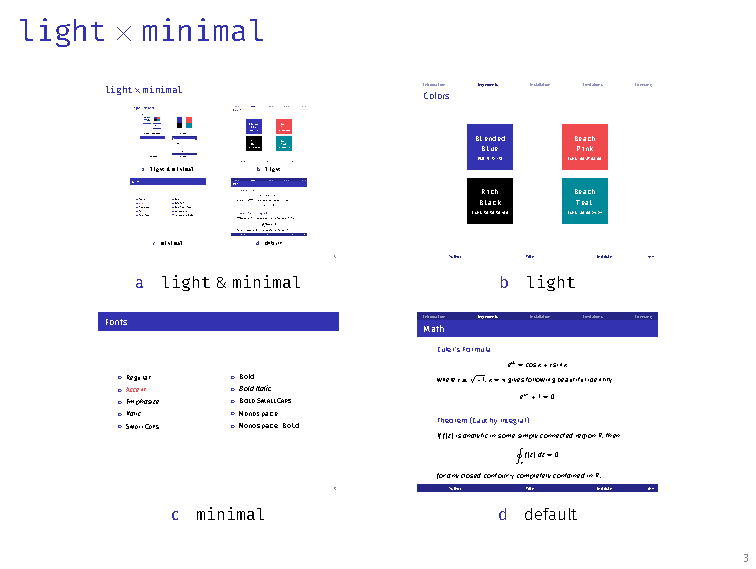
\includegraphics[width=.75\linewidth]{tutorial-style}
	\caption{\texttt{light} \& \texttt{minimal}}
	\label{fig:light-minimal}
\end{subfigure}%
\begin{subfigure}{.5\textwidth}
	\centering
	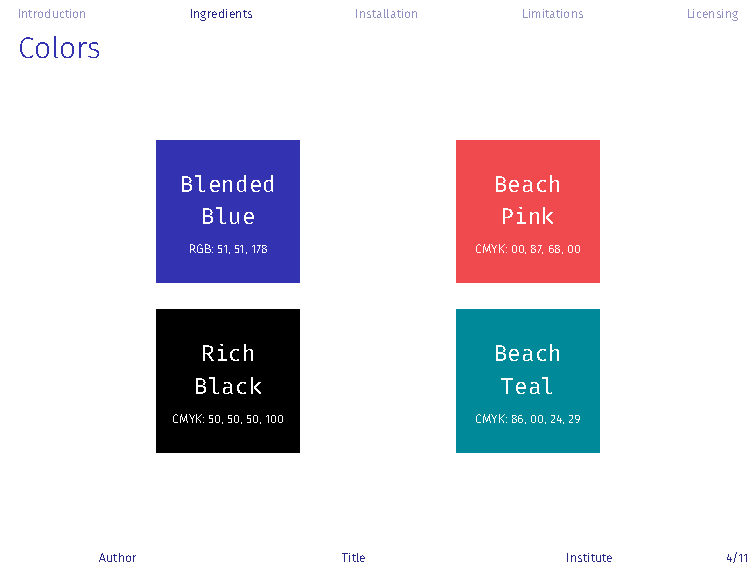
\includegraphics[width=.75\linewidth]{tutorial-light-color}
	\caption{\texttt{light}}
	\label{fig:light}
\end{subfigure}
\begin{subfigure}{.5\textwidth}
	\centering
	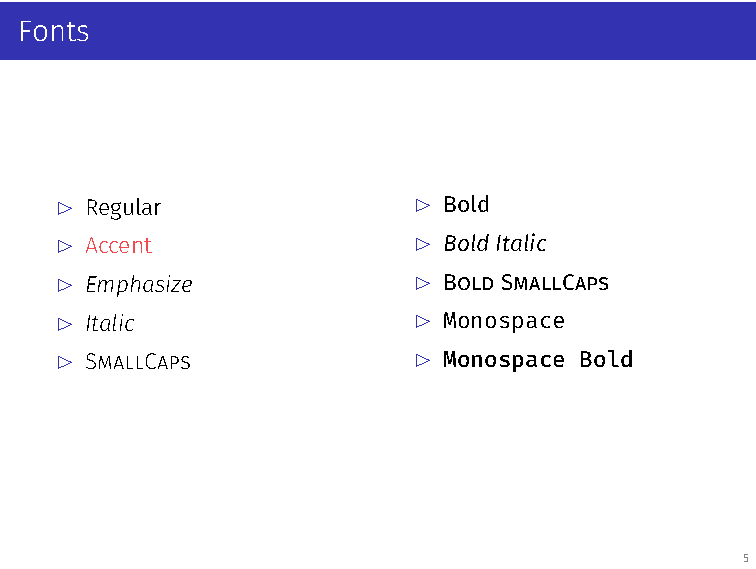
\includegraphics[width=.75\linewidth]{tutorial-minimal-font}
	\caption{\texttt{minimal}}
	\label{fig:minimal}
\end{subfigure}%
\begin{subfigure}{.5\textwidth}
	\centering
	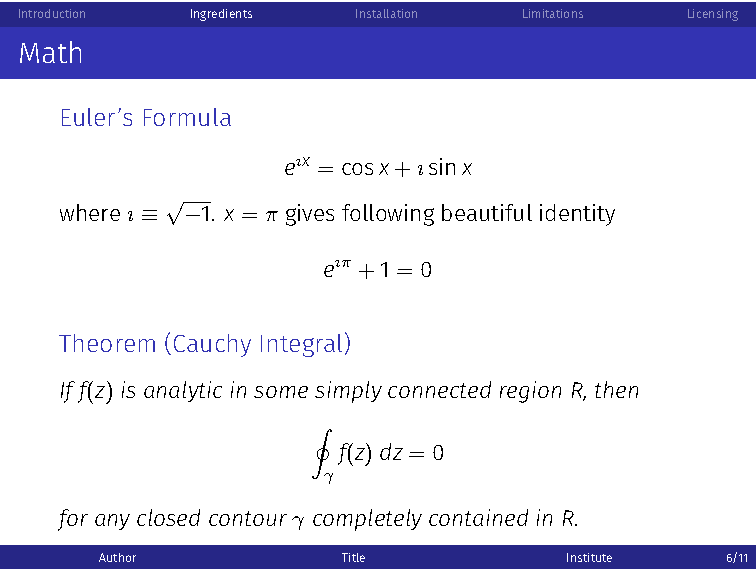
\includegraphics[width=.75\linewidth]{tutorial-default-math}
	\caption{default}
	\label{fig:default}
\end{subfigure}
%\caption{\texttt{light$\,\times\,$minimal} Style Option Gallery}
\label{fig:style}
\end{figure}
\end{frame}
%============================================================



%============================================================
%	INGREDIENT
%------------------------------------------------------------
\section{Ingredients}
%------------------------------------------------------------
\subsection{Colors}
%------------------------------------------------------------
\begin{frame}[c]{Colors}
\begin{columns}[c]

\begin{column}{12ex}
% Color Box: Beamer Blended Blue
\setbeamercolor{boxblendedblue}{bg=BlendedBlue,fg=white}
\begin{beamercolorbox}[wd=\linewidth,ht=9.5ex,dp=2.5ex,center,leftskip=2ex,rightskip=2ex]{boxblendedblue}%
\centering
	\texttt{Blended\\Blue}\par%
	\vskip\medskipamount%
	\tiny{RGB: 51, 51, 178}%\\\tiny{CMYK: 71, 71, 00, 30}
\end{beamercolorbox}
%\caption{\textcolor{BlendedBlue}{Main Structure}}
\vskip\bigskipamount

% Color Box: Northwestern Rich Black
\setbeamercolor{boxrichblack}{bg=RichBlack,fg=white}
\begin{beamercolorbox}[wd=\linewidth,ht=9.5ex,dp=2.5ex,center,leftskip=2ex,rightskip=2ex]{boxrichblack}%
\centering
	\texttt{Rich\\Black}\par%
	\vskip\medskipamount%
	\tiny{CMYK: 50, 50, 50, 100}%
\end{beamercolorbox}
%\caption{Normal Text}
\end{column}

\begin{column}{12ex}
% Color Box: `tutorial' Beach Pink
\setbeamercolor{boxbeachpink}{bg=BeachPink,fg=white}
\begin{beamercolorbox}[wd=\linewidth,ht=9.5ex,dp=2.5ex,center,leftskip=2ex,rightskip=2ex]{boxbeachpink}%
\centering
	\texttt{Beach\\Pink}\par%
	\vskip\medskipamount%
	\tiny{CMYK: 00, 87, 68, 00}%
\end{beamercolorbox}
%\caption{\alert{Alerted Text}}

\vskip\bigskipamount

% Color Box: `tutorial' Beach Teal
\setbeamercolor{boxbeachteal}{bg=BeachTeal,fg=white}
\begin{beamercolorbox}[wd=\linewidth,ht=9.5ex,dp=2.5ex,center,leftskip=2ex,rightskip=2ex]{boxbeachteal}%
\centering
	\texttt{Beach\\Teal}\par%
	\vskip\medskipamount%
	\tiny{CMYK: 86, 00, 24, 29}%
\end{beamercolorbox}
%\caption{\example{Example Text}}
\end{column}

\end{columns}
\end{frame}
%------------------------------------------------------------
\subsection{Typography}
%------------------------------------------------------------
\begin{frame}[c]{Fonts}
\begin{columns}[c]
\begin{column}{.5\textwidth}
\begin{itemize}
	\item Regular
	\item \alert{Accent}
	\item \emph{Emphasize}
	\item \textit{Italic}
	\item \textsc{SmallCaps}
\end{itemize}
\end{column}

\begin{column}{.5\textwidth}
\begin{itemize}
	\item \textbf{Bold}
	\item \textbf{\textit{Bold Italic}}
	\item \textbf{\textsc{Bold SmallCaps}}
	\item \texttt{Monospace}
	\item \texttt{\textbf{Monospace Bold}}
\end{itemize}
\end{column}
\end{columns}
\end{frame}
%------------------------------------------------------------
\begin{frame}{Math}
\begin{block}{Euler's Formula}
\vskip-\bigskipamount
\[e^{\imath x} = \cos{x} + \imath\sin{x}\]
where $\imath\equiv\sqrt{-1}$. $x=\pi$ gives following beautiful identity
\[e^{\imath\pi} + 1 = 0\]
\end{block}

\begin{theorem}[Cauchy Integral]
If $f(z)$ is analytic in some simply connected region $R$, then
\[\oint_{\gamma} f(z)\ \text{d}z = 0\]
for any closed contour $\gamma$ completely contained in $R$.
\end{theorem}
\end{frame}
%============================================================



%============================================================
%	INSTALLATION
%------------------------------------------------------------
\section{Installation}
%------------------------------------------------------------
\subsection{Theme and Typeface}
%------------------------------------------------------------
\begin{frame}{Theme \& Typeface}
\begin{block}{\theme\ Beamer theme}
	\begin{description}
	\item[frequent] put \texttt{sty} files into your Beamer theme \texttt{texpath}
	\item[occasional] leave them aside with your main \texttt{tex} file
	\end{description}
\end{block}

\begin{block}{Fira Sans typeface}
	\begin{description}
	\item[\texttt{xelatex}] \emph{recommend} to install \href{https://www.mozilla.org/en-US/styleguide/products/firefox-os/typeface/}{Mozilla Fira Sans typeface}
	\item[\texttt{pdflatex}] MiKTeX might install \texttt{FiraSans}, \texttt{FiraMono} and \texttt{newtxsf} packages on the fly
	\end{description}
\end{block}
\end{frame}
%------------------------------------------------------------
\subsection{Presentation}
%------------------------------------------------------------
\begin{frame}[fragile]{Presentation}
\begin{block}{Enable \texttt{light} and \texttt{minimal} \theme\ by loading}
\vspace*{-\bigskipamount}
\begin{verbatim}
\documentclass{beamer}
\usetheme[light,minimal]{tutorial}
\end{verbatim}
\vspace*{-\medskipamount}
Note that the options can be also passed to \texttt{beamer}.
\end{block}

\begin{block}{Customize colors by loading}
\vspace*{-\bigskipamount}
\begin{verbatim}
\setbeamercolor*{structure}{fg=main,bg=background}
\setbeamercolor{alerted text}{fg=alert text color}
\end{verbatim}
\vspace*{-\medskipamount}
\end{block}
\end{frame}
%------------------------------------------------------------
\begin{frame}{Packages}
\begin{table}
\ttfamily%
\begin{tabular}{rll}
	\hline\hline
	& \multicolumn{2}{c}{\textsf{Package}}\\
	\hline
	\theme\	& tikz	&\\
	\textsf{demo}
		& ccicons	& lstings\\
		& subcaption&\\
	beamer
		& amsmath	& amssymb\\
		& graphicx	& xcolor\\
		& enumerate	& hyperref\\
		& \multicolumn{2}{c}{\vdots}\\
	\hline\hline
\end{tabular}
\caption{Packages Loaded by \theme, Current Demo and Beamer}
\end{table}
\end{frame}
%============================================================



%============================================================
%	LIMITATIONS
%------------------------------------------------------------
\section{Limitations}
%------------------------------------------------------------
\begin{frame}[fragile]{Limitations}
\begin{itemize}
\item headline section navigation bar \emph{always} coexists with footline information
\item math and text font theme not yet carefully adjusted
\item \emph{fixed} frame numbering style
	\begin{itemize}
	\item frame number only for minimal
	\item otherwise shown as a fraction
	\end{itemize}
\item theme options \emph{cannot} \lstinline{\PassOptionsToClass} or \lstinline{\PassOptionsToPackage} through command line
\item common Beamer \texttt{compress} option untuned
\end{itemize}
\end{frame}
%============================================================



%============================================================
%	LICENSING
%------------------------------------------------------------
\section{Licensing}
%------------------------------------------------------------
\begin{frame}{Licensing}
Get the source of \theme\ and its demo from
\begin{center}\small
\href{http://github.com/jeffmxu/beamer-theme-tutorial}{\texttt{github.com/jeffmxu/beamer-theme-tutorial}}
\end{center}

\theme\ may be distributed and/or modified under the \href{http://www.latex-project.org/lppl.txt}{\LaTeX\ Project Public License} and the \href{http://www.gnu.org/licenses/gpl-3.0.txt}{GNU General Public License}.

\vskip\medskipamount

\theme\ \emph{itself} should also be licensed under the \href{http://creativecommons.org/licenses/by-sa/4.0/}{Creative Commons Attribution-ShareAlike 4.0 International License}.
%\vspace{-\bigskipamount}
\begin{center}\ccbysa\end{center}
\end{frame}
%============================================================



\end{document}%
